\documentclass[11.5pt]{sig-alternate} % sets document style to sig-alternate
% packages
% typesetting
%\usepackage{dirtytalk} % typset quotations easier (\say{stuff})
\usepackage{hanging} % hanging paragraphs
\usepackage[defaultlines=3,all]{nowidow} % avoid widows
\usepackage[pdfpagelabels=false]{hyperref} % produce hypertext links, includes backref and nameref
\usepackage{xurl} % defines url linebreaks, loads url package
\usepackage{microtype}
% layout
%\usepackage{enumitem} % control layout of itemize, enumerate, description
\usepackage{fancyhdr} % control page headers and footers
\usepackage{float} % improved interface for floating objects
%\usepackage{multicol} % intermix single and multiple column pages
% language
\usepackage[utf8]{inputenc} % accept different input encodings
\usepackage[english]{babel} % multilanguage support
% misc
\usepackage{graphicx} % builds upon graphics package, \includegraphics
%\usepackage{lastpage} % reference number of pages
%\usepackage{comment} % exclude portions of text (?)
\usepackage{xcolor} % color extensions
\usepackage[backend=biber, style=apa]{biblatex} % sophisticated bibliographies % necessary for HTML to display author info and date on abstract page
\usepackage{csquotes} % advanced quotations, makes biblatex happy
\usepackage{authblk} % support for footnote style author/affiliation
% tables and figures
\usepackage{tabularray}
%\usepackage{array} % extend array and tabular environments
\usepackage{caption} % customize captions in figures and tables (rotating captions, sideways captions, etc)
%\usepackage{cuted} % allow mixing of \onecolumn and \twocolumn on same page
\usepackage{multirow} % create tabular cells spanning multiple rows
%\usepackage{subfigure} % deprecated, support for manipulation of small figures
%\usepackage{tabularx} % extension of tabular with column designator "x", creates paragraph-like column whose width automatically expands
%\usepackage{wrapfig} % allows figures or tables to have text wrapped around them
%\usepackage{booktabs} % better rules
% dummy text
%\usepackage{blindtext} % blind text dummy text
%\usepackage{kantlipsum} % Kant style dummy text
%\usepackage{lipsum} %lorem ipsum dummy text
% other helpful packages may be booktabs, longtable, longtabu, microtype

\pagestyle{fancy} % sets pagestyle to fancy for fancy headers and footers

% header and footer
% modern way to set header image
\renewcommand{\headrulewidth}{0pt} % defines thickness of line under header
\renewcommand{\footrulewidth}{0pt} % defines thickness of line above header
\setlength\headheight{80.0pt} % sets height between top margin and header image, effectively moves page contents down
\addtolength{\textheight}{-80.0pt} % seems to affect the lower height. maybe only works properly if footer numbers enabled?
\fancyhf{}
\fancyhead[CE, CO]{
\includegraphics[width=\textwidth]{headerImage.png}}
% footer
%\fancyfoot[LE,LO]{Article Title Here \\ DOI: }% left footer article title and doi
%\fancyfoot[CE,CO]{{}} % center footer empty
%\fancyfoot[RE,RO]{\thepage} % right footer page numbers
%\pagenumbering{arabic} % arabic (1, 2, 3) numbering in footer

\hypersetup{colorlinks=true,urlcolor=blue} % sets link color to blue
\urlstyle{same} % sets url typeface to same as rest of text

% set caption and figure to italics, label bold, left align captions, does not transfer to HTML
\DeclareCaptionFormat{custom}
{
    \textbf{\textit{\large #1#2}}\textit{\large #3} % #1 is the "Table 1" or "Figure 1" part, #2 is the separator (":"), #3 is the caption
}
\captionsetup{format=custom}
\captionsetup{justification = raggedright, singlelinecheck = false}
 
\let\oldabstract\abstract
\let\oldendabstract\endabstract
\makeatletter
\renewenvironment{abstract}
{\renewenvironment{quotation}%
               {\list{}{\addtolength{\leftmargin}{1em} % change this value to add or remove length to the the default
                        \listparindent 1.5em%
                        \itemindent    \listparindent%
                        \rightmargin   \leftmargin%
                        \parsep        \z@ \@plus\p@}%
                \item\relax}%
               {\endlist}%
\oldabstract}
{\oldendabstract}
\makeatother

\begin{document}

\title{See3D: 3D Printing for People Who Are Blind}

\author[1]{\large \color{blue}Caroline Frances Karbowski}

\affil[1]{The Ohio State University}

\toappear{}
%% ABSTRACT
\maketitle
\begin{@twocolumnfalse} 
\begin{abstract}
\item 
\textit {Objects such as snowflakes, castles, and butterflies have become more than just words when explored as a 3D print. The founder’s passion for braille led to the creation of the program See3D, which organizes the printing and distribution of 3D printed models for people who are blind. 3D prints such as DNA, cells, animals, constellations, telescopes, historic landmarks, logos, and maps were created to fulfill requests by people who are blind for tactile learning tools. Recipients shared their feedback on how to improve the models, and the printing and distribution service. See3D seeks to spread awareness about accessibility by presenting at technology fairs and demonstrating to students how to work 3D printers. A culmination of research and interactions with people who are blind, blindness organizations, educators, and scientists on how 3D printing has impacted those who are blind and sighted added to the development of See3D. Currently, See3D is a tax-exempt, non-profit 501(c)(3) organization that has distributed more than 800 models to people in the United States and around the world, and continues to build its network of volunteers and collaborators.}
\\ \\
Keywords: 3D Printing, Blind, Visually Impaired, Low Vision, Tactile, Accessibility, STEM
\end{abstract}
\end{@twocolumnfalse}

%% AUTHOR INFORMATION

\textbf{*Corresponding Author, Caroline Frances Karbowski}\\
\href{mailto: karbowski.4@osu.edu }{(karbowski.4@osu.edu)} \\
\textit{Submitted January 14, 2020 }\\
\textit{Accepted February 11, 2020} \\
\textit{Published online February 24, 2020} \\
\textit{DOI:10.14448/jsesd.12.0006} \\
\pagebreak
\clearpage

\begin{large}
\section*{BACKGROUND}

\subsection*{Definition of Blindness}

For the purposes of the article, “blind” refers to someone who self-identifies as being blind, legally blind, visually impaired, having low vision, having sight loss, being partially sighted, etc., even with the use of corrective lenses.

\subsection*{3D Printing and it's Value in Education}

A 3D printed model is a 3-dimensional object that is made by extruding thin layers of heated plastic filament from a 3D printer to additively produce a tangible model from a drafted image (Martin et at., 2014). Tactile tools, such as braille, tactile graphics and 3D models, allow students who are blind to feel information that might otherwise be presented as a printed picture, or is too dangerous, large, small, or delicate to be touched in real life (Hasper et al., 2015; Horowitz \& Schultz, 2014; Koehler et al., 2018). Since creating tactile graphics can be labor intensive, students who are blind often use descriptions of visual content to access information (Sheppard \& Aldrich, 2001). However, images are a necessary component of the learning process (Hasper et at., 2015). It is important to be able to provide accurate tactile images that give students the information they need, and are also not expensive or labor-intensive to produce.

As 3D printers become more user-friendly, affordable, and upgraded they become more usable for people who may not have extensive technology experience (Söderberg, 2013). A person does not need to create their own computer aided design (CAD) of the object to 3D print a model, they can download a file shared online by who is already versed in the 3D design process (Kietzmann et al., 2015). With such a large online community of people of all ages and skills (Moilanen \& Vadén, 2013), there are many people who could be involved to create 3D printed models for people who are blind. The skills learned to create a 3D printed model can also be transferred to a variety of disciplines such as engineering, manufacturing, food, art, and health (Kietzmann et al., 2015), so people may be more likely to learn how to design and 3D print models. 3D printers themselves are also quite versatile, and the objects made on the printers can be beneficial for students who are blind and sighted, which allows for students of various levels of vision to use the same tactile learning tools (Hasper et al., 2015).

In a study comparing the understanding of geoscience concepts using tactile graphics and 3D printed models with students who are visually impaired, Koehler et al. (2018) found the students who used 3D printed models interacted more with the tool by handling the object in different angles and rearranging the pieces, while the students using the tactile graphics only recited the content provided by the braille labels to the researcher. A study on teachers’ views of tactile graphics found that students who are blind struggled to understand tactile graphics with unusual scale or perspective, like a 3-dimensional view, so teachers resorted to using models or real-life objects (Sheppard \& Aldrich, 2001). A benefit to 3D printing is that students could have an inexpensive model of virtually anything to use in conjunction with their tactile graphic. Students could develop their skills in interpreting graphics with the aid of a model, so when they encounter content that is only available in graphic form, they have the skills to better conceptualize the graphic. 

\subsection*{Inspiration and Development}

The founder of See3D, Caroline Karbowski, learn\-ed braille tactilely during middle school to alleviate dizziness while reading in the car. Without a personal connection to blindness, Karbowski was inspired to explore 3D printing after reading how visual science media could be made tactile using 3D printed models with braille labels (Kolitsky, 2014; Grice et al., 2015). With an opportunity to lead a showcase technology project for TechOlympics, a high school technology conference, Karbowski decided to incorporate braille, spare filament, and inspiration for 3D printing projects by creating See3D, which would organize the printing and distribution of 3D printed models for people who are blind. 

The showcase team developed a website, see3d.org (Figure 1) where model requests could be submitted to be printed by volunteers in the See3D network. Karbowski relied on meeting people who are blind and teachers of the visually impaired (TVI) to give feedback on the program, gain an understanding of what types of models would be useful for students who are blind, and spread the word of See3D’s offerings. Visits to museums that provide 3D prints of scanned artifacts and the Digital Fabrication Lab at the Indiana School for the Blind and Visually Impaired occurred to learn how to manage the production and quality of 3D printed models.

\begin{figure}[ht]
    \centering
    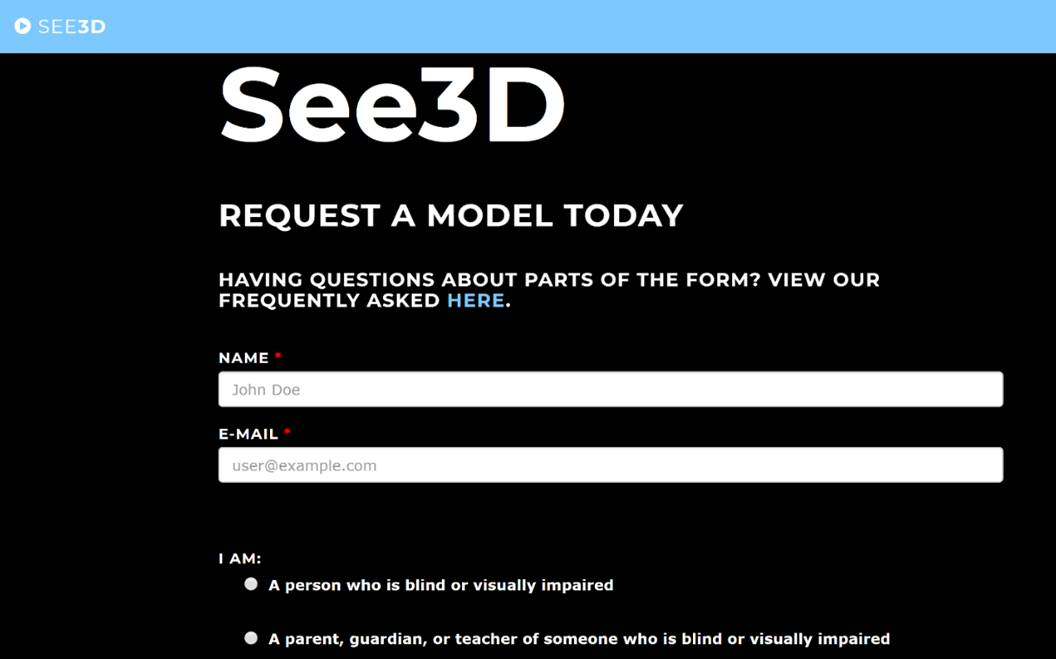
\includegraphics[width=1\linewidth]{1116_Fig1.jpg}
    \caption{Model Request form on see3d.org.}
\end{figure}

\section*{OPERATIONS}

\subsection*{Managing Domestic Requests}

See3D mainly fulfills requests by printing models published under Creative Commons or Public Domain Licenses, but also coordinates with volunteers to design new models like the screens of a smartphone (Figure 2), logos, and the stages of the butterfly life cycle (Figure 3). To mitigate the spread of personal information, models printed by volunteers are sent to a central See3D location where they are processed and sent to the recipient. Models can include a description of the model in braille, large print, or electronic format, as well as braille address labels on the shipping box. Braille labels can also be added to the model with label stickers or in some cases, 3D printed directly on the model (Figure 2). This way, people who are blind can identify their box from See3D and discover what their model has to offer independently.

\begin{figure}[ht]
    \centering
    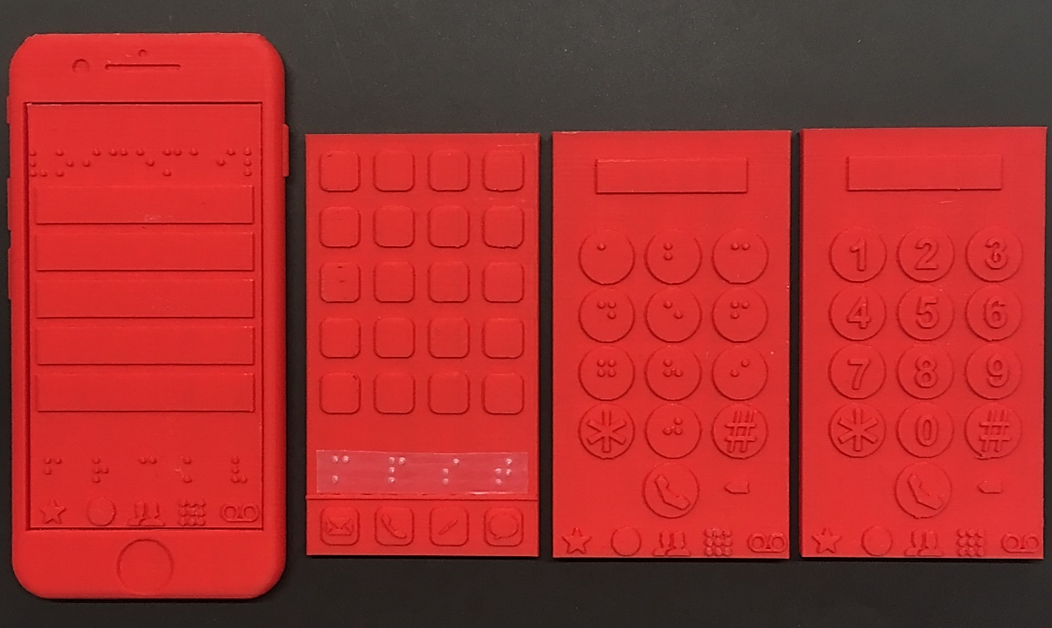
\includegraphics[width=1\linewidth]{1116_Fig2.png}
    \caption{3D Printed model of a smartphone body and interchangeable screens for voicemail, home apps, and number pad with 3D printed braille, clear braille labels, and 3D printed numerals. Requested model designed by See3D volunteer, Jamie Varney, 2019.}
\end{figure}

\begin{figure}[ht]
    \centering
    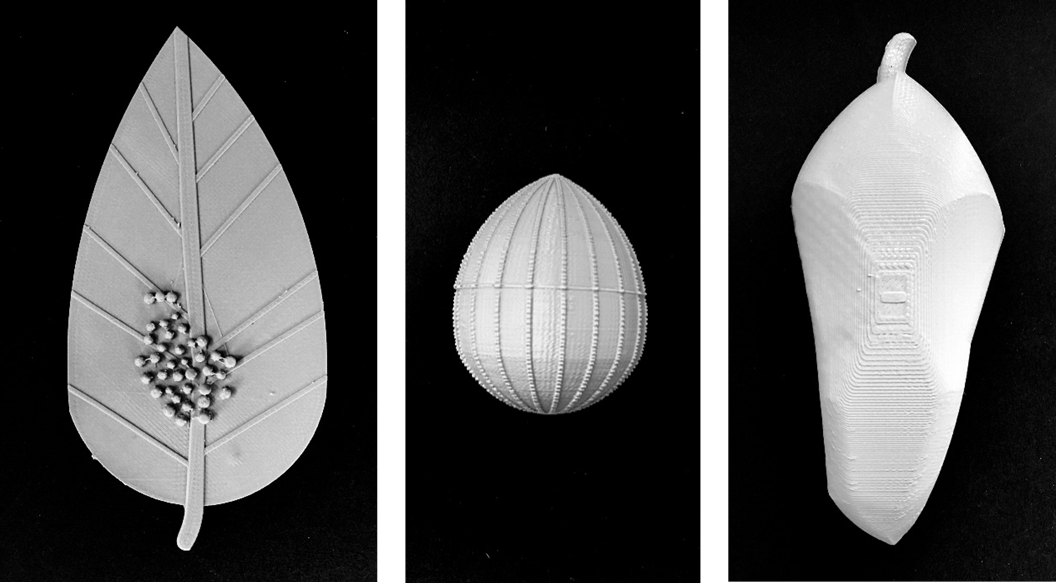
\includegraphics[width=1\linewidth]{1116_Fig3.png}
    \caption{Models of butterfly eggs on a leaf, monarch egg, and chrysalis. Requested models designed by See3D volunteer, Jamie Varney, 2019.}
\end{figure}

\subsection*{International Requests}

For international requests, See3D has sent stereo-lithography (STL) files to be printed by the recipient, and has given models to people who are traveling. Using these processes, models have been sent to Canada, Empower Blind People in Kyrgyzstan, Familias Especiales in Nicaragua, and the Ministry of Education Resource Unit for the Blind and Visually Impaired in Guyana. A few volunteers outside the United States have contacted See3D and offered to print for people in their country, and See3D is hoping to expand the number of volunteers to accommodate more international requests. 

\section*{PURPOSE}

\subsection*{Social Impact and Networking}

See3D seeks to provide more educational resources for people who are blind, as well as make positive societal change about the attitudes of blindness. Rowland \& Bell (2012) found being a friend or even having a conversation with someone who is blind can increase favorable views and expectations about people who are blind. See3D creates an opportunity for people who are blind and sighted to meaningfully interact when the person who requested the model and the person providing the model engage in model feedback. See3D raises awareness about blindness at maker events where they provide an experience for guests to touch models, write braille, and explore tactile graphic books that correlate to 3D models. These events are often attended by people who enjoy 3D printing, so volunteers frequently sign up at the event to contribute to the designing and printing of requests. By networking with 3D model designers, schools, libraries, companies, and nonprofit organizations at maker expos, See3D continues to build on its mission to connect and collaborate with people who are blind and sighted through 3D printing.

\subsection*{Community Involvement}

In addition to individual orders, See3D coordinates group requests for schools, organizations, events, and conferences. Examples include the Ohio Braille Challenge in Cincinnati, Ohio, the 2019 BELL Academy of the National Federation of the Blind (NFB) of Ohio in Columbus, Ohio, and the Newport Aquarium in Newport, Kentucky.

During the 2018-2019 school year, the Ohio State School for the Blind (OSSB) Model Club contacted See3D about a project to refurbish and display their model collection of historic landmarks such as the Taj Mahal, Parthenon, The Great Pyramid of Giza, and the United States Capitol Building, made by artists in the 1930s as part of the Works Project Administration (Writers' Program (Ohio), 1941). The school only owns one large model of each landmark, so they asked to collaborate on printing smaller models for students to grasp the general shape before exploring the larger historic models for more detail (Figure 4). See3D has been working with the Model Club to share how to download available STL files and maintain their 3D printers. By involving students in the 3D printing process, students can practice using access technology and can take ownership of the tactile materials they are providing for themselves and their classmates. 

\begin{figure}[ht]
    \centering
    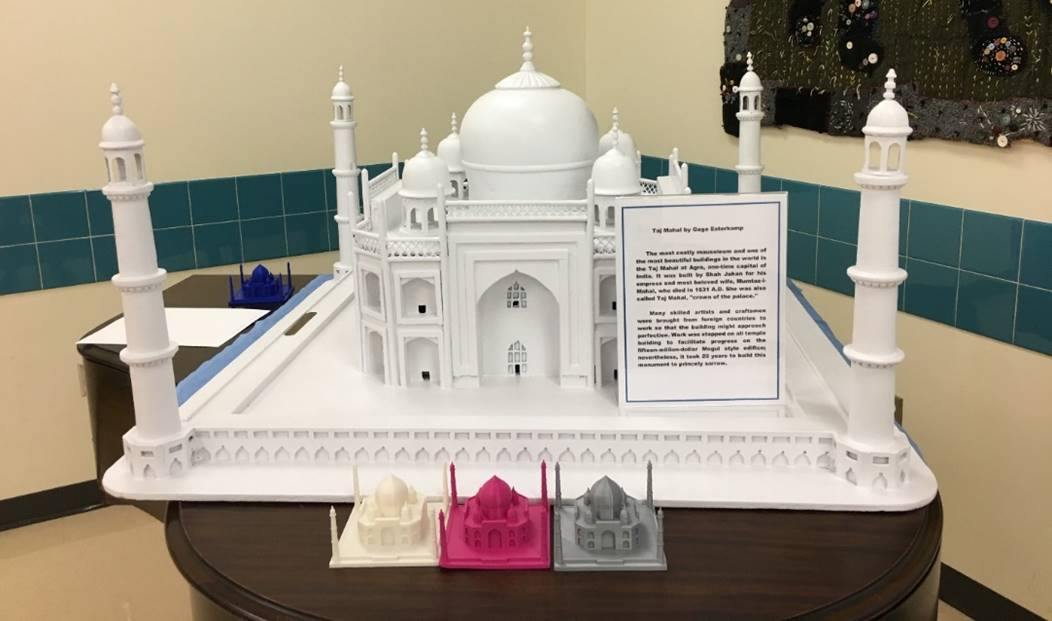
\includegraphics[width=1\linewidth]{1116_Fig4.jpg}
    \caption{Taj Mahal model from the Ohio State School for the Blind historic landmark model collection with four smaller 3D printed Taj Mahal models (dodo2000, 2015) printed by students in the OSSB Model Club. A large print and braille description written by students is also included to give historical context for the model.}
\end{figure}

\subsection*{Advocating for Accessibility}

The purpose of See3D is to connect people who enjoy 3D printing with those who could benefit from touching a tactile model. See3D hopes that as awareness is spread about the need for 3D printing to be accessible, more 3D printing companies will make modifications to their software and devices to make them more compatible for users who are blind. With the advancement of refreshable tactile graphic displays, See3D is optimistic that people who are blind could feel the progress of their virtual objects in order to adjust the design before making a print (N. Mckenzie, personal communication, August 31, 2019). 
\\ \\
\section*{RESPONSE}

General responses from recipients were positive, and many have since requested additional models. Recipients often contact See3D with their gratitude and feedback, such as the testimonial from an Associate Professor at Bowling Green State University, who requested models of constellations.

\begin{quote}
“It is the speed and immediacy that delights me; the quick uncovering of hidden things. The sudden, silent, precise unfurling of knowledge under my hands. And, I know things with confidence that were only shrouded ideas to me before” (personal communication, October 10, 2019).
\end{quote}

By conversing with people who are blind about how they interpret a concept before and after touching a model, new perspectives can be shared and appreciated among See3D volunteers and recipients of models. After touching a model of a Cinderella castle, one recipient who is a M.S. Cognitive Neuroscience Ph.D. candidate, stated,

\begin{quote}
“I had a vague idea what a castle looked like in terms of the base. The top and towers were completely new to me; I'd always heard of towers and castles but didn't imagine the towers were a part of the castle. I thought the third dimension looked like a triangle like houses do. I also didn't know bridges were attached to castles” (personal communication, May 20, 2019).
\end{quote}

Many recipients stated they gained a different perspective and a new understanding of a concept after touching the model, and were interested in learning how to print models. 

\subsection*{Future Directions}

Currently, the See3D team consists of three undergraduate second-year students: Caroline Karbowski, Garrett Carder, and Emily Kiehl. They collaborate to develop the website, connect with people who are blind, print and design models, develop marketing strategies, and manage legal responsibilities. Karbowski is a biology major, and See3D is not part of the coursework required for the degree. Karbowski plans to continue to incorporate See3D in a science career after graduation.   

See3D is interested in collaborating with educational researchers and nonprofit and for-profit organizations to distribute, evaluate the accuracy, and research the efficacy of the models. See3D also plans to ask for feedback from volunteers before and after printing a model, to see if their perceptions of blindness have been affected by their involvement with the organization. Asking recipients for suggestions on how to improve the models will continue to be implemented. As word spreads, See3D hopes to reach more international partners, so more model processing groups can be created to distribute models to a wider audience. 

Over the last three years, See3D has distributed more than 800 models to people who are blind. Looking forward, See3D is working to make a login system for people who request, design, and print models. Recipients of models would only need to enter their contact information once, and they could receive updates on the progress of their model. Volunteers would be able to see a running feed of requests, and could select the model they would like to undertake as well as update their progress, so other volunteers know what print jobs are currently available. See3D also plans to utilize social media platforms to announce design requests, and raise awareness. By building a community of people interested in 3D printing and accessibility, See3D strives to bring a new understanding of the world’s concepts and surroundings through touch.  

\section*{ACKNOWLEDGMENTS}

See3D would like to acknowledge the following organizations: the GE Additive Education Program, Jane Goodall’s Roots \& Shoots, Vora Ventures, IC3D, GeckoTek 3D Printer Build Plates, Polar3D, the Clovernook Center for the Blind \& Visually Impaired (Cincinnati), the C-SUN Assistive Technology Conference, The Ohio State University Entrepreneurial Business Law Clinic, and The Ohio State University Innovation Studio.

\end{large}
\clearpage
\section*{REFERENCES}\par 

\begin{hangparas}{0.25in}{1}
Dodo2000. (2015, July). Taj Mahal. Retrieved from \url{https://www.thingiverse.com/thing:934616}

Grice, N., Christian, C., Nota, A., \& Greenfield, P. (2015). 3D Printing Technology: A Unique Way of Making Hubble Space Telescope Images Accessible to Non-Visual Learners. \textit{Journal of Blindness Innovation and Research, 5}(1). \url{https://doi.org/10.5241/5-66}

Hasper, E., Windhorst, R. A., Hedgpeth, T., Van, T. L., Gonzales, A., Martinez, B., Hongyu, Y., Farkas, Z., \& Baluch, D. P. (2015). Methods for creating and evaluating 3D tactile images to teach STEM courses to the visually impaired. \textit{Journal of College Science Teaching, 44}(6), 92-99.

Horowitz, S. S., \& Schultz, P. H. (2014). Printing space: Using 3D printing of digital terrain models in geosciences education and research. \textit{Journal of Geoscience Education, 62}(1), 138-145.

Kietzmann, J., Pitt, L., \& Berthon, P. (2015). Disruptions, decisions, and destinations: Enter the age of 3-d printing and additive manufacturing. \textit{Business Horizons, 58}(2), 209-215. \url{https://doi.org/10.1016/j.bushor.2014.11.005}

Koehler, K. E., Wild, T. A., \& Tikkun, S. (2018). Implications of 3-D printing for teaching geoscience concepts to students with visual impairments. \textit{Journal of Science Education for Students with Disabilities, 21}(1), 49-81. \url{https://doi.org/10.14448/jsesd.10.0004}

Kolitsky, Michael A. (2014). 3D printed tactile learning objects: Proof of concept. \textit{Journal of Blindness Innovation and Research, 4}(1). \url{https://doi.org/10.5241/4-51}

Martin, R. L., Bowden, N. S., and Merrill, C. (2014). 3d printing in technology and engineering education. \textit{Technology and Engineering Teacher, 73}(8), 30-35. 

Moilanen, J., \& Vadén, T. (2013). 3D printing community and emerging practices of peer production. \textit{First Monday, 18}(8). \url{https://doi.org/10.5210/fm.v18i8.4271}

Rowland, M. P., \& Bell, E. C. (2012). Measuring attitudes of sighted college students towards blindness. \textit{Journal of Blindness Innovation and Research, 2}(2). \url{http://dx.doi.org/10.5241/2F2-24}

Sheppard, L \& Aldrich, F.K. (2001). Tactile graphics in school education: Perspectives from teachers. \textit{British Journal of Visual Impairment, 19}(3), 93-97. \url{https://doi.org/10.1177/026461960101900303}

Söderberg, Johan. (2013). Automating amateurs in the 3D printing community: Connecting the dots between ‘deskilling’ and ‘user-friendliness’. \textit{Work Organisation, Labour \& Globalisation, 7}(1), 124-139. \url{https://www.jstor.org/stable/10.13169/workorgalaboglob.7.1.0124}

Writers' Program (Ohio). (1941). Models for the blind. Columbus, Ohio. Retrieved January 12, 2020, from \url{http://hdl.handle.net/2374.OX/186736}

\end{hangparas}
\end{document}
